\documentclass[11pt]{article}
\usepackage[a4paper,left=3cm,right=3cm,top=3cm,bottom=4cm]{geometry}       
\geometry{letterpaper}                   
\usepackage{hyperref}
\usepackage[official]{eurosym}
\usepackage{listings}
\usepackage{pdfpages}
\usepackage{graphicx}
\usepackage{amssymb}
\usepackage{epstopdf}
\usepackage{natbib}
\usepackage{amssymb, amsmath}
\usepackage{url}
\usepackage{graphicx}
\usepackage{wrapfig}
\usepackage[skip=0pt]{caption}
\usepackage{tabularx}
\setlength\parindent{0pt}
\newcolumntype{C}{>{\centering\arraybackslash}X}
\usepackage[onehalfspacing]{setspace}
\captionsetup[figure]{font=small,labelfont=small}
\newcommand*{\captionsource}[2]{%
  \caption[{#1}]{%
    #1%
    \\\hspace{\linewidth}%
    \textbf{Source:} #2%
  }%
}

\usepackage{float}
\DeclareGraphicsRule{.tif}{png}{.png}{`convert #1 `dirname #1`/`basename #1 .tif`.png}

\usepackage[
    backend=biber,
    style=numeric,
    sorting=none
]{biblatex}
\addbibresource{bibliography.bib}


%\title{Title}
%\author{Name 1, Name 2}
%\date{date} 

\begin{document}


\thispagestyle{empty}

\begin{center}

\includegraphics[width=5cm]{ETHlogo.eps}

\bigskip


\bigskip


\bigskip


\LARGE{Complex Social Systems:\\ }
\LARGE{ Modelling Agents, Learning, and Games\\}

\bigskip

\bigskip

\small{Project Report}\\

\bigskip

\bigskip

\bigskip

\bigskip


\begin{tabular}{|c|}
\hline
\\
\textbf{\LARGE{The Influence of Cyclists on Traffic}}
\\
\hline
\end{tabular}
\bigskip

\bigskip

\bigskip

\LARGE{Nils Egger, Sophia Herrmann, Jan Hochstrasser, Jannick Schröer, Alexander Sotoudeh}



\bigskip

\bigskip

\bigskip

\bigskip

\bigskip

\bigskip

\bigskip

\bigskip

Zurich\\
December 2022\\

\end{center}
\newpage

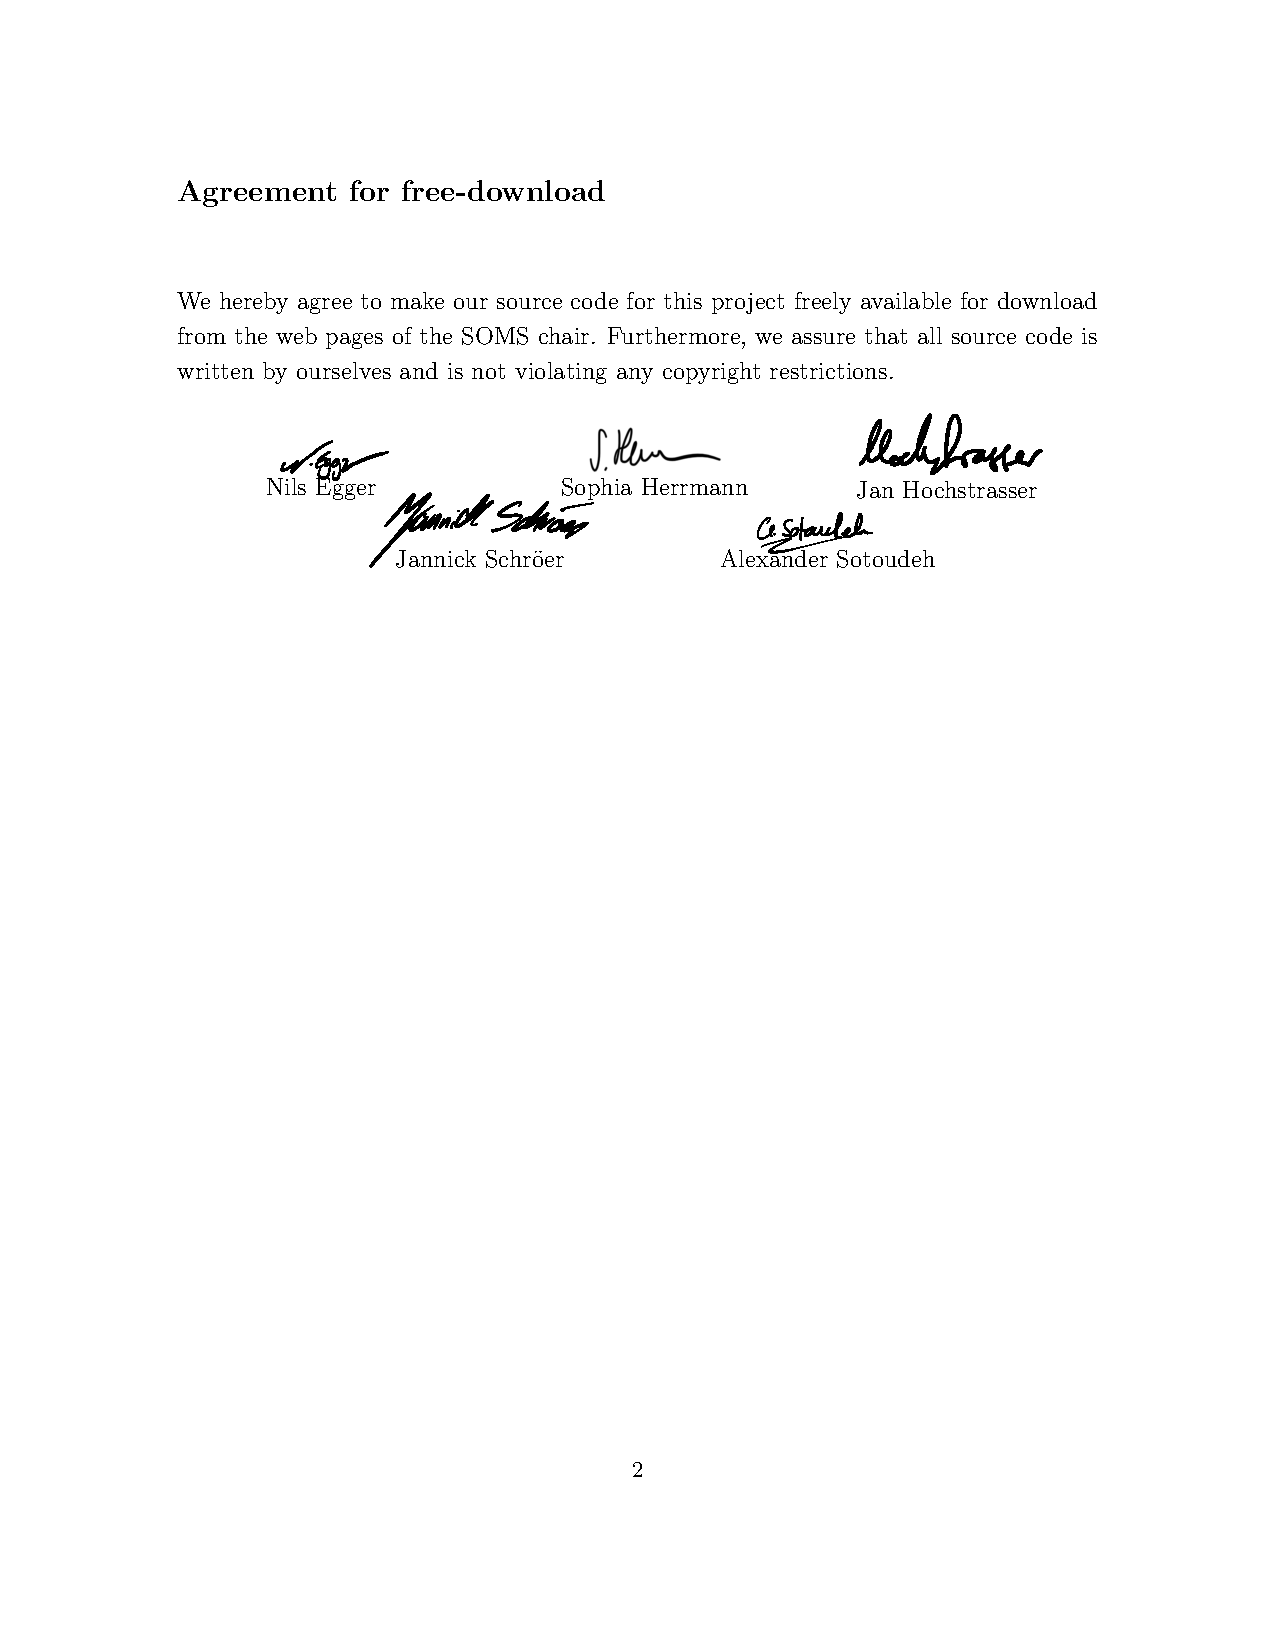
\includepdf[pages=-]{AgreementSignatures-full.pdf}
%%%%%%%%%%%%%%%%%%%%%%%%%%%%%%%%%%%%%%%



% IMPORTANT
% you MUST include the ETH declaration of originality here; it is available for download on the course website or at http://www.ethz.ch/faculty/exams/plagiarism/index_EN; it can be printed as pdf and should be filled out in handwriting
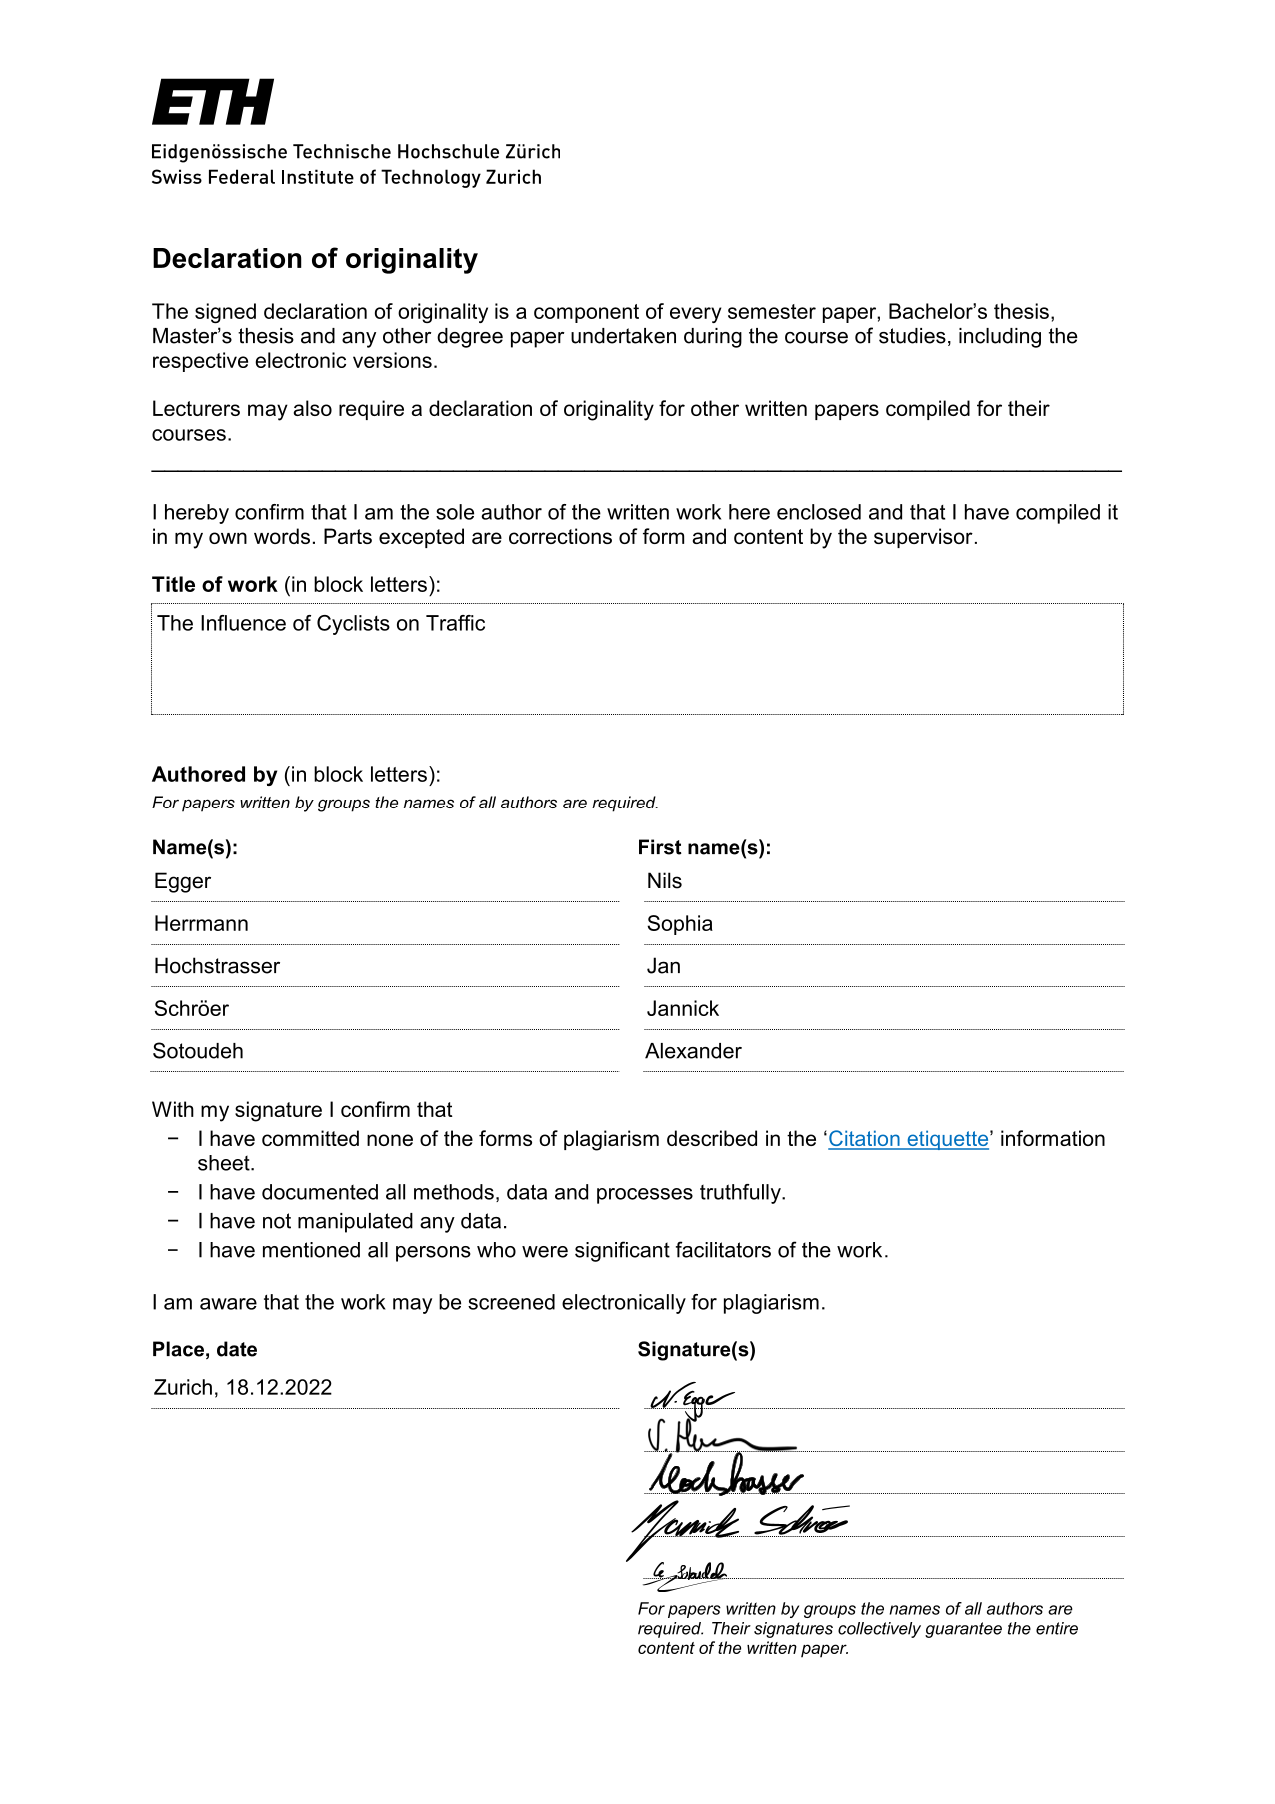
\includepdf[pages=-]{declaration-originality-signatures-full.pdf}

%%%%%%%%%% Table of content %%%%%%%%%%%%%%%%%

\tableofcontents

\newpage

%%%%%%%%%%%%%%%%%%%%%%%%%%%%%%%%%%%%%%%




\section{Abstract}
Due to the pandemic and also the city of Zurich pushing for more environmentally friendly transportation, bicycle usage has seen a growth in recent years. This report entails a description of an Agent Based Model, which aims to simulate the traffic of Zurich under the influence of a varying amount of cyclists on the road. The model consists of an environment, given by the road network accessible by cars and bicycles, depicted by agents. It found that higher percentages of bicycles with a consistent absolute amount of agents does not result in any significant changes. Part of this could be caused due to certain abstractions made, which are mentioned in section \ref{abstractions}.\\
Nevertheless, the absence of significant changes in traffic flow, density or average speed, as described in section \ref{results}, is not necessarily something bad. This also allows the conclusion that an increase in cyclists does not cause an increase in congestions or travel time of commuters. Therefore it is not a solution to traffic jams, but does also not cause more. This allows an increase of cyclists in traffic, if aspired for other reasons, without risking a more congested city. These reasons could include a safer and quieter city, as well as less environmental pollution.

\section{Individual contributions}
Sophia was in charge of research and related papers, gathering the data and the initial filtering round. Jan then further cleaned up the data and parsed it into a viable input form. This included generating the agents, that were then fed into the model. Nils wrote a preliminary draft of the code. Alexander then took the draft, expanded upon it, optimised it to be run in parallel on RACKlette, a High Performance Computing Cluster. Jannick created a web-interface to visualise the model, which was integral to debugging and also the final presentation. The report was written by Jan, Alex and Sophia, with graphs generated by Jannick. The presentation was made primarily by Jan and Sophia.
We would also like to thank Faveo Hörold, who gave us some advice on getting the simulation to run on the HPC Cluster.



\section{Introduction}
\subsection{Motivations}
%% small talk
Traffic is omnipresent in everyday societal life. The average swiss person traverses an average distance of 36,8 km per day.  \cite{mobil}
The biggest hindrance in daily commute and travel is the emergence of traffic jams and road congestions. `The impact of personal time lost in congestion includes not only the stress disruption to family life, but perhaps even more also important it includes the opportunity cost of that lost time.' \cite{congestion}. Congested traffic has many detriments, and results in many unfavorable side effects, next to the delay to travel time. 

%% accidents
Congested traffic leads to higher accident rates. A 10\% reduction in congestion can lead to a 3.4\% reduction in car accidents. \cite{SanchGoz}  Congested traffic also leads to so called stop-and-go traffic, which increases the occurrence of rear-end collisions. \cite{golob} Collisions and accidents then further disrupt the traffic, resulting in higher congestions and more delays, essentially forming a vicious cycle.

%% health detriment (+ enviromental impact?)
Traffic jams also negatively impact the environment and human health. Higher traffic volume results in higher levels of nitrogen dioxide, in an almost linear relation. \cite{zhang} Elevated $NO_2$ concentrations pose a health risk. It has been linked to increased respiratory diseases and heart issues. \cite{goudarzia} This leads to dangers for the people living close to highly used roads, as well as for the users of said roads. The additional time spent on the road due to congested traffic further fuels the risk to the passengers' health.

%% costs
Finally, traffic congestions lead to a tangible cost, carried by the government and/or private people. This cost manifests itself in different ways. These costs can stem from accidents, which as explained above, are increased by congestion. In the EU, passenger car accidents alone resulted in 210.2 billion euros of damages. \cite{eurocomm} The aforementioned environmental impact of congestions can also be tied to a cost, produced by health effects, crop loss, biodiversity loss, and material damage. A kilogram of nitrogen dioxide produced by transport is estimated to cost 21.3 euros on average. With Switzerland having produced 35 781 tonnes through transport in 2015, one can very clearly see how the additional pollution results in higher costs \cite{swissno2}. Lastly, congestions give rise to an aptly named ``congestion cost". The publications office of the European Union organizes these into two categories; congestion costs and scarcity costs, defined as follows: `A ‘congestion cost’ arises when one scheduled service delays another.' \cite{eurocomm} and `A ‘scarcity cost’ arises where the presence of a scheduled service prevents another scheduled service from operating, or requires it to take an inferior slot.' \cite{eurocomm} respectively. Together, these resulted in a cost of 208.3 billion euros produced by passenger cars in the EU. \cite{eurocomm}
\\
%%zurich bicycles
In an effort to reduce the negative effects propagated by excessive traffic usage, the city of Zurich proposed a strategy to reduce car traffic and emission titled `Stadtverkehr 2025: Strategie für eine stadtverträgliche Mobilität'. \cite{strategie25} As of 2021, regular cyclists made up 12\% of road users. \cite{bericht21} One of the primary goals of this campaign is to increase the percentage of bicycle users in regards to total traffic. This spawned further campaigns, such as the `Velostrategie 2030'. By expanding and improving the existing road network, the city of Zurich aims to promote cycling as an environment friendlier alternative to driving. \cite{velo2030}

%%corona bicycles
Bicycle usage has also seen a sharp increase due to the pandemic. With quarantines and lock downs, the usage of bicycles has seen a surge in popularity. With a 40\% increase for work related trips and a 60-80\% increase for leisure trips \cite{covid, mobis}, a trend towards the bicycle becomes clear. This raises the question of how bicycles influence traffic.

%%related works
\subsection{Related Papers}
Related papers have already studied the effect of bicycle lanes on car traffic. \cite{bikelanes}
This report and underlying project aim to investigate the effect varying numbers of cyclists have on the travel time of motorists with help of an Agent Based Model. Agent Based Modelling lends itself very well for traffic flow modeling. It's intuitive to model different vehicles as agents, making decisions based on environmental factors and the actions of other Agents. Other benefits of using ABM include the fact that it is a very flexible model. It is easy to add more agents or change certain behaviors, without having to redesign the entire model. \cite{bazghandi} As such, it is no surprise that ABM is already a widely spread medium for traffic simulations. The specialization for each topic then stems from the way different papers define their agents' behavior. Some papers assign drivers different driving styles, based on aggressiveness, confidence, etc \cite{abmfortraffic}, whereas other papers opt for more homogeneous driving styles. \cite{sanfran} Finally, since many decisions made by the agents happen simultaneously, ABM is very suitable for parallelism and for being run on High-Performance-Computers. \cite{cuda} Like others before us, we capitalized on this, in order to get more performance out of our model. By simulating scenarios with different levels of bike usage, our model could help policymakers and city planners better understand the potential impacts of promoting cycling as a transportation option. This information can potentially be valuable in further developing the existing strategies to encourage more people to use bicycles, which might help reduce congestion and improve the overall efficiency of the transportation system. 









\section{Description of the Model}
 
\subsection{Environment}
\begin{wrapfigure}[18]{r}{0.5\textwidth}
  \centering
    \vspace{-0.4cm}
  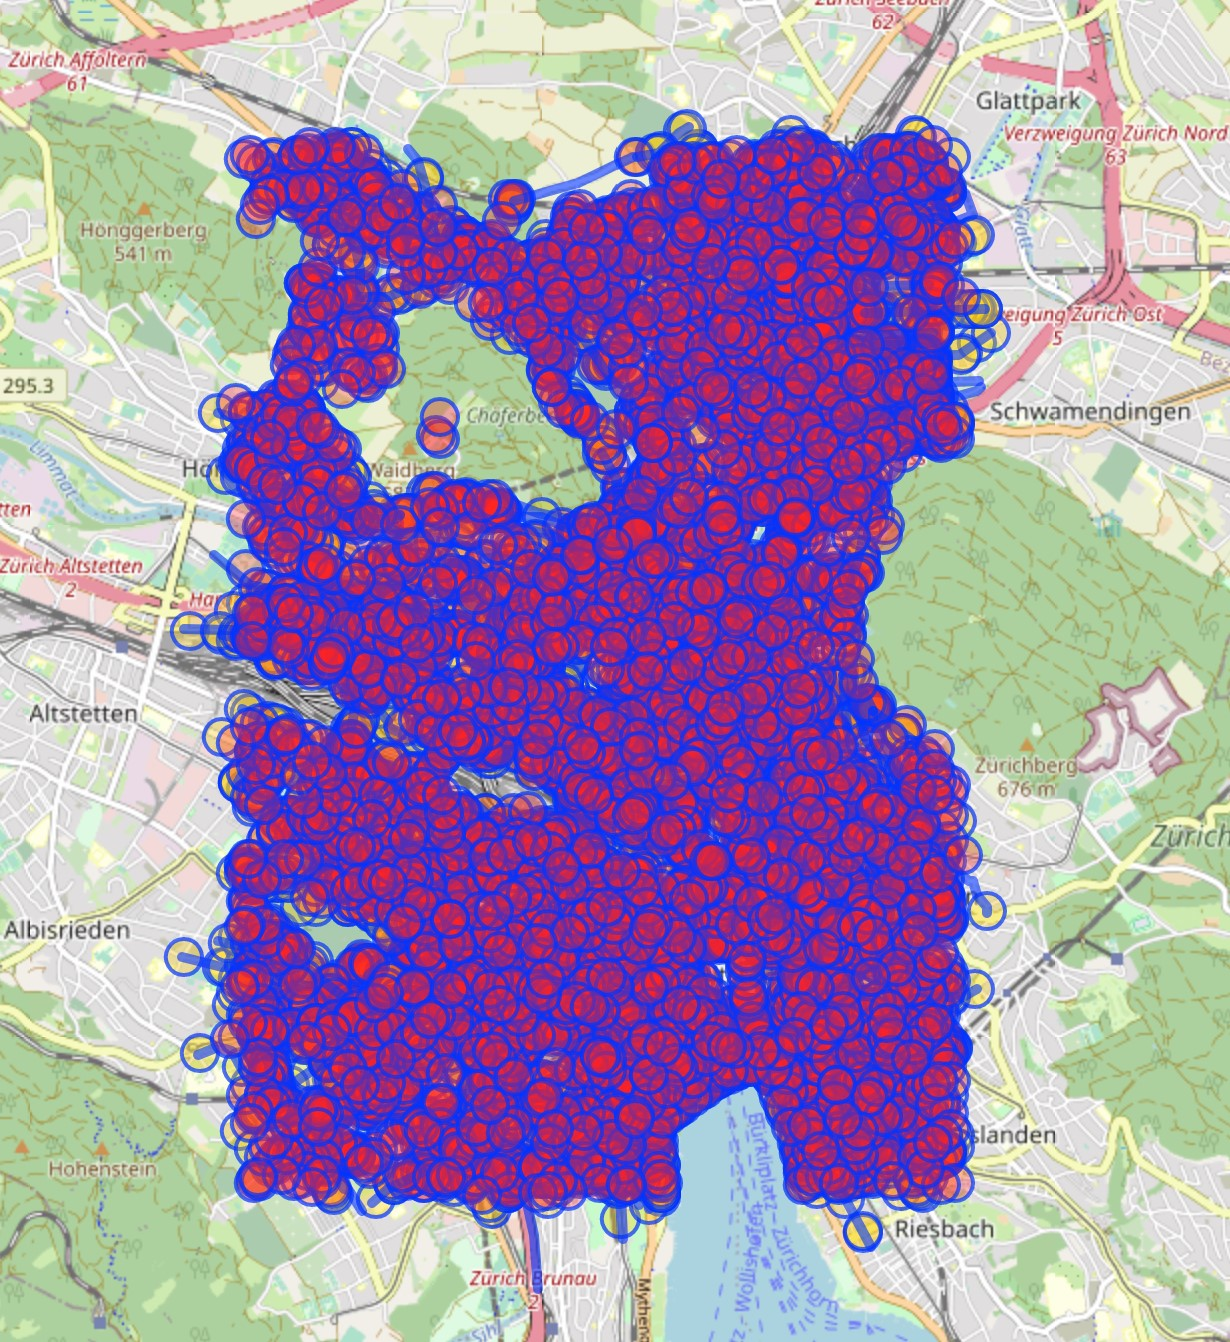
\includegraphics[width=\linewidth]{./figures/road-network.jpg}
  \captionsource{Modelled Road Network}{Screenshot taken from result of using our query in Overpass Turbo}\label{network}
\end{wrapfigure}

To understand the impact of bicycles on the traffic flow of cars we decided to make use of an Agent Based Model.  The realtime decisions made every day by thousands of travelers translate well into decisions to be made by Agents. Furthermore, traffic, and in particular car traffic, is constrained to roads, which makes for a very well defined environment. Our model environment is based on the road network of Zurich. Specifically, this model is constrained to the inner city of Zurich, using approximately a square of 4.5 by 8.9 kilometers of road network (see Fig.: \ref{network}).\\
The road network used contains streets ranging from larger highways and main roads such as the ``Limmatstrasse" but also smaller, more private roads.\\
In the model itself, the road network is split into streets and the intersections they are connected to. Both streets and intersections possess unique attributes. 

\subsubsection{Intersection}
The intersections are modeled as nodes in a graph with certain attributes. These attributes consist of an ID, a longitude and latitude attribute to denote its position, as well as which roads are incoming and outgoing. All intersections are modelled to be controlled through traffic lights. These are solely time controlled.

\subsubsection{Streets}
Each street is modeled as a directed edge between two intersections/vertices. Next to its ID, each street is uniquely determined by its start and end points, as well as its type. The type refers to the vehicle type which can use the road, which is ``bike", ``car" or ``mixed". Therefore there is at most one edge available for each agent type between two pairs of vertices.\\
A street has several attributes. One is the number of lanes, which is assumed to be one as default, in case there is no further information in the raw data. The other attributes are the speed limit, which is assumed to be 50 km/h as a default, as well as the length of the road, which is calculated using the coordinates of its endpoints.

\subsection{Agents}\label{agentDesc}
\subsubsection{General Attributes}
The agents consist of two types, cyclists and cars. Each agent has a start and end intersection, which determines the start and end point of its journey. Furthermore, an agent has several attributes determining the behavior. The attributes have an interval for cyclists and for cars, which it is uniformly chosen out of (see Tab.: \ref{tab:agentAttr.}). Each agent possesses an additional attribute, that tells it at what time to start its journey. This value is given in seconds. 

\begin{table}[H]
\begin{center}
\begin{tabularx}{\linewidth}{C|C|C|C|C|C}
    & \textbf{Length} ($m$) & \textbf{Maximum Velocity} ($km/h$) & \textbf{Accel-} \textbf{eration} ($m/s^2$) & \textbf{Decel-} \textbf{eration} ($-m/s^2$) & \textbf{Acceleration Exponent}\\
    \hline
    \textbf{Cars} & $[3.5, 5]$ & $[100, 250]$ & $[1.5, 5]$ & $[2, 6]$ & $[8, 12]$\\
    \hline
    \textbf{Bicycles} & $[1.5, 2.5]$ & $[10, 35]$ & $[0.5, 1.5]$ & $[1, 3]$ & $[8, 12]$
\end{tabularx}
\caption{Possible Ranges for Agent Attributes}\label{tab:agentAttr.}
\end{center}
\end{table}
\vspace{-0.75cm}
The agents are generated hourly and for each agent in this hour, the exact time of departure is uniformly chosen. The absolute amount of agents per hour is calculated relative to the area of the map. We assume that for every 4'000$m^2$ of the map, one agent spawns per hour. This number was chosen, since in 2022 there where 182'805  motorized vehicles registered in the city of Zurich. \cite{carAmount} About 57\% of daily kilometers is absolved through motorized individual transport. \cite{verhalten} Therefore, we made the assumption, that every second vehicle is moved once a day, resulting in around 90'000 agents spawned over the course of the simulation. Most of them travel in the span of around 12 hours, which we made the length of the simulation. This leaves us with one agent spawned per hour and 4'000$m^2$, to achieve a total of approximately 90'000 agents over twelve hours on the used map.
\subsubsection{Agent Behaviour}
Every agent wishes to travel from its start to end point as quickly as possible. At the beginning of the simulation, the shortest paths between all nodes are calculated. The agent chooses this path for their journey and uses the appropriate streets to travel from intersection to intersection. On the street, the agent accelerates or decelerates to maintain a safe distance from the next agent. If the street has multiple lanes, the agent will choose the lane with the most space available. Bikes are required to stay in the right lane on large streets unless the street is marked as bike-only. Furthermore, agents can overtake other agents (i.e. a car overtakes a slower bike), provided there is a high enough difference in speed and there is a free lane on the overtaking agent's left. The equation to describe the motion of the agents is the following: \cite{helbl}
\begin{align*}
\dot{x}_\alpha &= v_\alpha\\
\dot{v}_\alpha &= a\left[ 1 - \left( \frac{v_\alpha}{v_0}\right)^\delta - \left(\frac{s^*(v_\alpha, \Delta v_\alpha)}{s_\alpha} \right)^2 \right]
\end{align*}

Where $s^*(v, \Delta v)$ is the dynamic desired distance defined by:
\begin{equation*}
s^*(v, \Delta v) = s_0 + v T +  \frac{v\Delta v}{2\sqrt{a\cdot b}}
\end{equation*}

The above-used variables have the following meanings, where $\alpha$ denotes our agent:
\begin{align*}
x_\alpha &= \text{ distance from agent to next intersection}\\
v_\alpha &= \text{ velocity to be achieved by agent}\\
v_0 &= \text{ current speed}\\
\Delta v_\alpha &= \text{ difference in velocity either to next agent or to intersection}\\
a &= \text{ acceleration of agent}\\
b &= \text{ deceleration of agent}\\
\delta &= \text{ acceleration coefficient}\\
s_\alpha &= \text{ current distance to next object}\\
s_0 &= \text{ minimum distance to next object}\\
T &= \text{ time}
\end{align*}



\section{Implementation}
The code created for the implementation of this simulation, as described in this section, can be found on GitHub: \href{https://github.com/AliSot2000/CSSMALG}{https://github.com/AliSot2000/CSSMALG}.
\subsection{Data Gathering}
\subsubsection{Map Creation}
The first step to building our model was gathering the relevant data. The data for the road network and thus the environment came from OpenStreetMap (OSM). OSM represents the real world by storing physical objects as nodes, ways and relations, and then describing and attributing them with the help of tags. 
OSM provides an API called Overpass API, which allows a user to fetch data based on the Overpass Query Language (Overpass QL). The language is built around the concept of creating a set of data, so consequently, the operations are also meant for sets, such as unions, intersections and complements. The following query was used to get our set of data:
\begin{lstlisting}
[out:json][bbox:47.36, 8.50, 47.42, 8.56];
        (
            way[highway=primary];
            way[highway=secondary];
            way[highway=trunk];
            way[highway=tertiary];
            way[highway=service];
            way[highway=residential];
        )->.a;
        (.a;>;);
out;
\end{lstlisting}

The map is bounded by the coordinates [47.36, 8.50, 47.42, 8.56], going from south, to west, to north, to east. It proved to be immensely difficult to efficiently filter out all roads not accessible by cars, so a level of abstraction was chosen to guarantee that no road within the environment was inaccessible to cars. This is at the cost of some smaller roads missing, that might also serve as pedestrian walkways. This is done by the different road types that are considered, which are mentioned in the ``highway" tag in the query above. \\
After the initial data gathering, the data had to be further cleaned and converted into an input usable by the simulation. This includes the removal of not connected roads. Furthermore, if there is a node on a street, which is not connected to any other street, it is removed and not treated like an intersection. These nodes mostly symbolize things like pedestrian crossovers, and are therefore not relevant to us, as mentioned in section \ref{abstractions}.\\
In order to achieve this, we wrote a PHP script, which takes the raw OSM data, received as a JSON file, and gives out the cleaned JSON file as an output.

\subsubsection{Agent Generation}
The agents are also generated using PHP. The nodes of the newly created map are read in. For each agent that is to be created two intersections are chosen randomly as start and end points. Furthermore, the values for the attributes are uniformly picked, as mentioned in section \ref{agentDesc}.\\
There is an option to add in a JSON file containing node pairs, that are not reachable from one another. These are filtered out during the agent generation to not cause issues during the simulation.\\
Agent files are generated for several percentages of bikes in traffic. The percentages increase from 0\% to 20\% in two percentage point increments. For each percentage 10 agent files are generated. Due to the random generation of the files, this should even out irregularities, enabling more reliable results.

\subsection{Model Programming}
% TODO ÜBERARBEITEN

Considering the scale we wanted to achieve in our simulation, we chose the programming language C++ combined with the parallel library CUDA. The simulation is capable of simulating real world street data or artificial data created by our own web interface. Our model was programmed with modularity in mind. Different executables generate intermediate results, which can then be reused without having to recalculate all the different stages again. This reduces total computational cost.

\subsubsection{Shortest Path Tree Calculation - PrecalcSPT}
Upon receiving the cleaned map data, or an artificial map from the web interface, we calculate a shortest path tree (or SPT) with PrecalcSPT for every distinct pair of intersections. The edge weights are defined to be the length of the the street which that edge represents. We do this using the Floyd Warshall algorithm. We used it due to its simplicity of implementation. Because it is a matrix-based algorithm, it is very suitable for parallelization. For our map of Zurich, that contained approximately 19'500 edges and 9'000 nodes, the computation time was around 15 minutes. PrecalcSPT generates the SPT and exports it in a base64 file. The reason the shortest path trees are stored like this, are limitations with the JSON library used, as well as issues with the maximum size of strings.

\subsubsection{Simulation - Simulate}
Simulate is the primary work horse of our simulation. It handles the simulation in the fastest manner possible. While it can be used in conjunction with PrecalcSPT and GenerateAgents to generate a visualization, its main purpose is the generation of the traffic statistics, such as traffic density, flow, etc., from the simulation of the real world map. Simulate was specifically optimized to run as fast as possible on a multi-core CPU. \\
All agents start out in a sorted insertion queue, waiting for the model time to match their personal insertion time. As soon as the time matches and the designated start intersection has space, an agent is moved to that intersection. On the street, the agent is able to ``see" up to the next crossing at most. Given the distance to the next obstacle and its velocity, the agent accelerates / decelerates to reduce the distance between himself and the next obstacle. If an agent cannot move (e.g. due to a congestion), he increases a counter which denotes the time it spent waiting. \\
Once an agent arrives at an intersection, there's a threshold of 0.6m after which an intersection can decide how to route an agent. An agent can be routed in two different ways: 

\paragraph*{Destination:}
Simply picking the next street in the path designated by the SPT.

\paragraph*{Yield Approximation:}
The yield approximation is very aggressive. In every time step the intersection moves to the next inbound road in a circular fashion and sends that agent to the next road he want's to go on if there's space.\\
\newline
Once an agent arrives at their destination, the arrival time is stored and the agent is removed from the simulation. The arrival intersection keeps track of all the actors which have already arrived there. \\
In order to speed up the simulation, the majority of it is parallelized. The only sequential parts are the data loading and movement. Independent updates like moving the agents, searching for available space in roads and checking for new agents that want to leave an intersection, can be done concurrently. 

\subsubsection{Web Interface}
The web interface was originally thought as a way to create maps for the simulation. This would have been for the purpose of testing the simulation and the path-finding algorithms. We decided to use the interface not only for creating maps for testing, but also for displaying the calculated simulations. This gave our team a lot of flexibility and allowed us to test the simulation with different parameters and different maps. A lot of bugs were easily found as we could see how the agents acted. The web interface was fully made with HTML, JavaScript and jQuery.

\subsection{Visualizing}
The visualizing onto graphs was fully done using the data output by the simulation. We imported the relevant data into a MongoDB Database and used MathPlotLib to visualize the data we were interested in.


\begin{frame}[containsverbatim, fragile]{Average Speed}
        \vspace{-0.2cm}
        \begin{figure}
		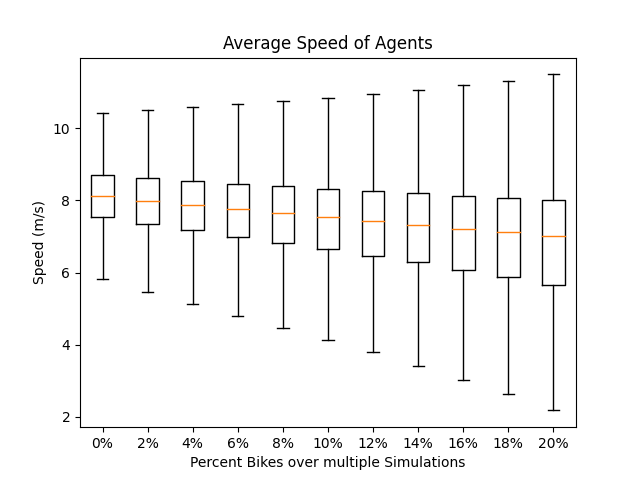
\includegraphics[width=0.65\textwidth]{Images/avg_speed_agent.png}
	\end{figure}
\end{frame}

\begin{frame}[containsverbatim, fragile]{Traffic Flow}
\vspace{-0.2cm}
        \begin{figure}
		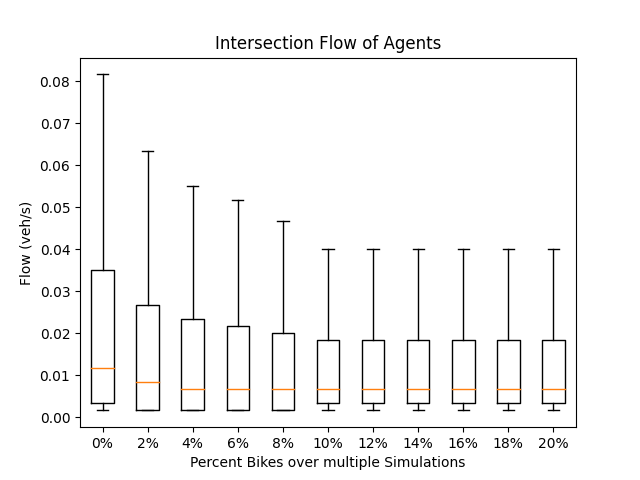
\includegraphics[width=0.65\textwidth]{Images/intersection_flow_agent.png}
	\end{figure}
\end{frame}

\begin{frame}[containsverbatim, fragile]{Traffic Density}
\vspace{-0.2cm}
        \begin{figure}
		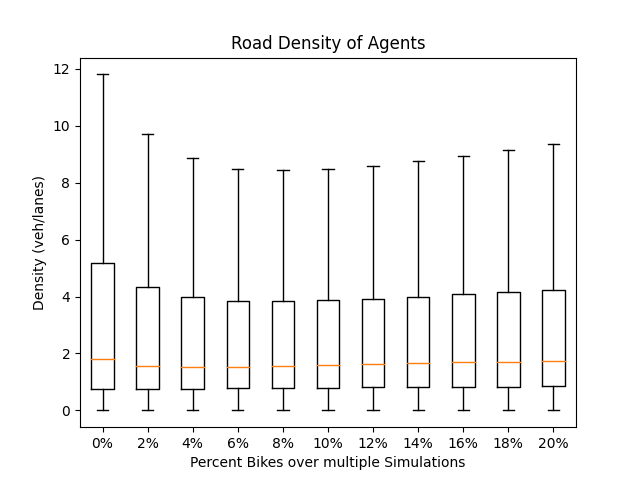
\includegraphics[width=0.65\textwidth]{Images/road_density_agent.png}
	\end{figure}
\end{frame}

\section{Conclusion and Outlook}
\subsection{Conclusion} \label{summary}
As was seen in section \ref{results}, the results suggest the amount of cyclists in traffic does not have much affect on the average speed, density or flow of road users. The slight decrease in average speed is negligable for the short distances, which are travelled inside of a city like Zurich. This would make a difference of mere seconds on a trip. When looking at the density or flow in section \ref{density} and \ref{flow}, the amount of cyclists  does not suggest a meaningful relief from congestions, nor is the average speed increased. All in all, our results show no meaningful influence of an increase in cyclists on traffic. Nevertheless, there are other reasons to move away from motorised individual transport to bicycling or usage of public transport, like a quieter and more peaceful city and less environmental pollution. These goals are also worth pursuing, especially since an increase in cyclists does not suggest a worsening of the traffic situation in our simulation.\\
However, as seen and described in section \ref{avg-speed}, there are some slight trends. The differences between the different values are small and negligible. Due to the abstractions mentioned in section \ref{abstractions}, not accounting for some behavior of agents and other influential factors on traffic in our model, combined with only slight trends in the result, this does not allow for the results to be transferred to reality one-to-one.\\

\subsection{Outlook}
There are many things a future model could expand upon. An immediate and natural expansion would be to include other users of the road network, such as public transport and pedestrians. Furthermore, bicycling is heavily dependant on environmental factors, such as weather and seasons. While the weather is somewhat difficult to model, the seasons could be an interesting way to account for a coarser trend. \\
Other than that, further improvements could be made by expanding the existing model with more detail. This could include more realistic routes for the agents, by regarding existing traffic when calculating routes, instead of precomputing all the shortest routes solely based on the length of the roads. This would be possible by calculating the routes iteratively and regard the current traffic situation when fixing the edge weights. By choosing an appropriate time step for the iterations, this would allow for a balance between computational resources needed and the accuracy of the model. More complex behavior of the agents is also a point, where current abstractions could be eliminated. This could include overtaking on opposite lanes if free and not only, if the immediate left lane is free. Furthermore the driving styles could be randomized a bit further and not only be dependent on the given attributes.\\
Another possibility to make the model more accurate, is to add more realistic travel data. Although hard to get, meaningful travel data, like trends in the start and destination of inner city travel or the amount of agents over the course of a day could drastically increase the significance of results.  Finally, one could always expand the model simply by using a more precise road network. 


\section{References}
\subsection*{Bibliography}
\addcontentsline{toc}{subsection}{Bibliography}
\printbibliography[heading=none]

\addcontentsline{toc}{subsection}{List of Figures}
\listoffigures

\addcontentsline{toc}{subsection}{List of Tables}
\listoftables


\end{document}  
